\documentclass[fleqn]{jbook}
\usepackage{physpub}

\begin{document}
\let\b\mathbf
\def\para{$p$-H$_2$}
\def\ortho{$o$-H$_2$}
\def\eV{\mathrm{eV}}
\begin{question}{問題9}{立川}
水素分子の衝突によるパラ水素分子(\para)からオルト水素分子(\ortho)への化学反応(水素原始間の結合の組替え)に関連して、以下の設問に答えよ。
\begin{enumerate}
\item まず、水素分子をボルン・オッペンハイマーの断熱近似で考えよう。2つの陽子がそれぞれ$\b R_1$, $\b R_2$の位置に固定されている時の2電子系の基底状態エネルギー(断熱ポテンシャル)を$U_2(|\b R_1-\b R_2|)$と書こう。これは$|\b R_1-\b R_2|=R_0=1.40a_{\mathrm{B}}$ ($a_{\mathrm{B}}$はボーア半径)で最小となる。
陽子の運動を考える際には、この$U_2(|\b R_1-\b R_2|)$が陽子間相互作用ポテンシャルを与えることになる。なお、陽子の質量$M$は電子の質量$m$の1840倍である。
\begin{enumerate}
\item 2つの陽子の運動は重心運動と相対運動に分離できるが、このうち、相対運動に関するシュレーディンガー方程式を$U_2(|\b R|)$を使って書き下せ。但し、$\b R=\b R_1-\b R_2$である。
\item この方程式の角度成分に注目し、相対距離$|\b R|$は$R_0$と近似して、2陽子系の回転運動のエネルギー固有値$E_L$を$M$や$R_0$を使って表わせ。
ここで、$L=0,1,2,\ldots$である。
さらに、$\hbar^2/ma^2_{\mathrm{B}}=27.2\eV=3.2\times10^5$Kであることを使って、
$E_1-E_0$の値をK単位で求めよ。
\item 陽子は核スピンが$\frac12$であるが、\para とは2つの陽子の核スピンが反平行なもの(合成核スピンが0)、\ortho とはそれが平行のものである。それぞれの分子について、許される$L$の状態とその縮重度を述べよ。
\item 合成核スピンがゼロの基底状態にある水素分子と重水素分子 D$_2$について解離エネルギーをはかったところ、それぞれ 4.46eV, 4.54 eVであることが分かった。これから、水素分子のゼロ点振動エネルギーの大きさを具体的に求めよ。なお、重水素の原子核は質量が$2M$で、核スピンは1である。
\end{enumerate}
\item 次に、H$+$H$_2$系を考えよう。この場合の断熱ポテンシャルは核スピンには依らず、図\eqhref{adiabatic}(a)で定義された3つの変数、$R_a$, $R_b$ および$\theta$の関数となる。図\eqhref{adiabatic}(b)--(d)には、その断熱エネルギー$U_3(R_a,R_b,\theta)$の代表的な$\theta$の値における様子が等高線の形で表示されている。なお、各等高線の値は最小値(図中の黒丸で示した点における$U_3(R_a,R_b,\theta)$の値で、これはあまり$\theta$にはよらない。)から測ったエネルギーの増加分(eVの単位)である。
この図を参考にしながら、次の各問に答えよ。
\begin{figure}[b]
\begin{center}
%\includegraphics[scale=.75]{2000phy9-1-reduced.eps}
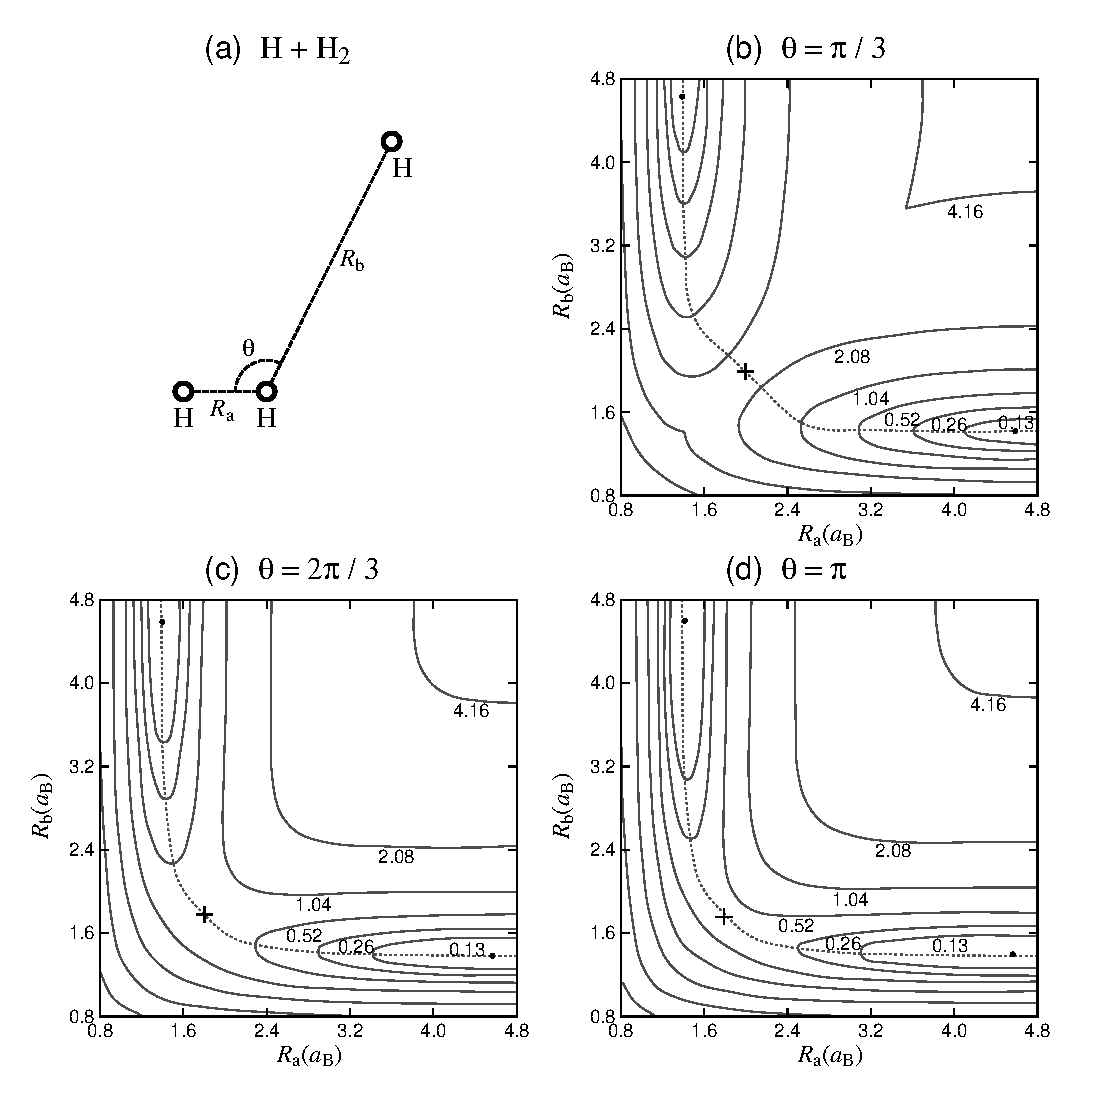
\includegraphics[scale=.75]{2000physQ9_1.eps}
\end{center}
\caption{H$+$H$_2$系における断熱ポテンシャル\eqname{adiabatic}}
\end{figure}
\begin{enumerate}
\item $U_3(R_a,R_b,\theta)$を最小にする$\{R_a,R_b\}$の組のうち、
小さいほうはほぼ$R_0$と等しいので、$U_3(R_A,R_B,\theta)$の最小値は自由な水素原子のエネルギーと$U_2(R_0)$の和にほぼ等しいことがわかる。しかしながら、より詳しく見ると、実際の最小値はその和よりも約 2meV ほど低くなっている。この余分の引力エネルギーが何に由来するかを述べよ。
\item $R_a$と$R_b$がともに無限大となるとき、$U_3(R_a,R_b,\theta)$は$\theta$によらずに、ある一定値に近づく。その一定値の具体的な値を求めよ。
\item 図\eqhref{adiabatic}(b)--(d)で、黒丸の点と十字印の点とを貫く点線経路に沿ったエネルギー変化の様子を参考にして、ビーム上の水素原子を打ちこんで基底状態にあるパラ水素分子と衝突させることによって得られるオルト水素分子がもっとも良く検出されるのは、元のビームの方向から見てどの角度であるか、推論せよ。
\item この化学反応を気相中300Kで行うと、270Kで行った場合よりも3.6倍の収量の増加が見られた。このことから、この反応に関連した活性化エネルギー$E_a$を eV の単位で求めよ。ただし、$\ln 3.6=1.3$である。得られた$E_a$と図\eqhref{adiabatic} (b)--(d) の十字印で示された点におけるエネルギーの値との関係を議論せよ。
\end{enumerate}
\end{enumerate}
\end{question}
\begin{answer}{問題9}{}
\begin{enumerate}
\item 
\begin{enumerate}
\item 陽子の重心まわりの換算質量は$M/2$なので、シュレーディンガー方程式は\[
E\psi(\b R)=-\frac{\hbar^2}{M}\frac{\partial^2}{\partial\b R^2}\psi(\b R)+U_2(|\b R|)\psi(\b R)
\]である。
\item 上式ハミルトニアンは球対称なので波動関数を角運動量の固有値で展開すれば\[
\frac{\hbar^2 L(L+1)}{r^2 M}-\frac{\hbar^2}{2Mr^2}\frac{\partial}{\partial r}
r^2\frac{\partial}{\partial r}+U_2
\]となる。振動状態による$r$部分のエネルギー期待値の変化を小さいと考えれば、
回転運動によるエネルギー固有値は\[
\frac{\hbar^2 L(L+1)}{MR_0^2}
\]と求まる。特に\[
E_1-E_0=\frac{\hbar^2 (1\cdot 2-0\cdot 1)}{MR_0^2 }
=\frac{\hbar^2}{ (1840 m) (1.40a_{\mathrm{B}})^2}
=\frac{3.2\times 10^5}{1840\cdot 1.40^2}\mathrm{K}
=88.7\mathrm{K}。
\]
\item 陽子はフェルミオンだから、2陽子系の波動関数は軌道部分とスピン部分をともに交換したとき符号を変えねばならぬ。
軌道波動関数は$L$の偶奇に従って符号を変え、
スピン波動関数は全スピン$0$のときが奇で全スピンが$1$のときは偶だから、
\begin{itemize}
\item \ \para: $L=0,2,4\ldots$ 縮重度はそれぞれ$1,5,9\ldots$;
\item \ \ortho: $L=1,3,5\ldots$ 縮重度はそれぞれ$3,7,11\ldots$
\end{itemize}となる。
\item $U_2(R)$の最小まわりを$U_2(R_0)+\frac12k(R-R_0)^2+\cdots$と展開すると
その中を動く質量$M$の振動子のゼロ点エネルギーは\[
\frac\hbar2\sqrt{\frac{k}{M}}
\]である。
よって合成核スピン0の水素分子の基底状態のエネルギーは$(\hbar/2)\sqrt{k/M}$。
一方でスピン1ふたつからスピン0をつくるとスピン波動関数は対称だから
(なぜならベクトルふたつを内積してスカラーをつくる操作は対称だから)
合成核スピンゼロの重水素分子の基底状態の角運動量は$L=1$である。よって\[
\frac\hbar2\sqrt{\frac{k}{M}}+4.46\eV
=\frac\hbar2\sqrt{\frac{k}{2M}}+\frac{\hbar^2\cdot\  1\cdot 2}{2MR_0^2}+4.54\eV
\]以上より$(\hbar/2)\sqrt{k/M}=0.299\eV$。
\end{enumerate}
\item 
\begin{enumerate}
\item 水素原子が水素分子に近づくことによって双方の中間状態に誘起される双極子間の相互作用によるエネルギー。van der Waals 力。
\item 3つの水素原子のそれぞれの電子が1s 状態にあることによるエネルギー。
すなわちRydberg 定数の3倍で $-3\times13.6\eV=-40.8\eV$。
\item 越えなければならないポテンシャルの峠がもっとも低いのは$\theta=\pi$のときである。角が$\theta$の方向から近づいて角が$\theta$の方向へぬけて行くと
$\pi-2\theta$だけ曲がるので、結局ビームの入射方向から$180^\circ$まわって
もと来た方向へ生成分子は飛んでいくと考えられる。
\item 平衡反応ではなくて、一方向に反応が進むとして、
越えなければならないエネルギーの峠を$E_a$とすると、
収量は$\exp(-E_a/kT)$に比例すると考えられる。
$\exp(-E_a/k(300\mathrm{K})/\exp(-E_a/k(270\mathrm{K}))=3.6$
から$E_a=0.30\eV$と求まる。
これは図の(d)の峠の高さとほぼ一致しているので、
この峠を抜けて反応が起こったと考えられる。
\end{enumerate}
\end{enumerate}
\end{answer}


\end{document}
